\documentclass[tikz,border=10pt]{standalone}

\begin{document}
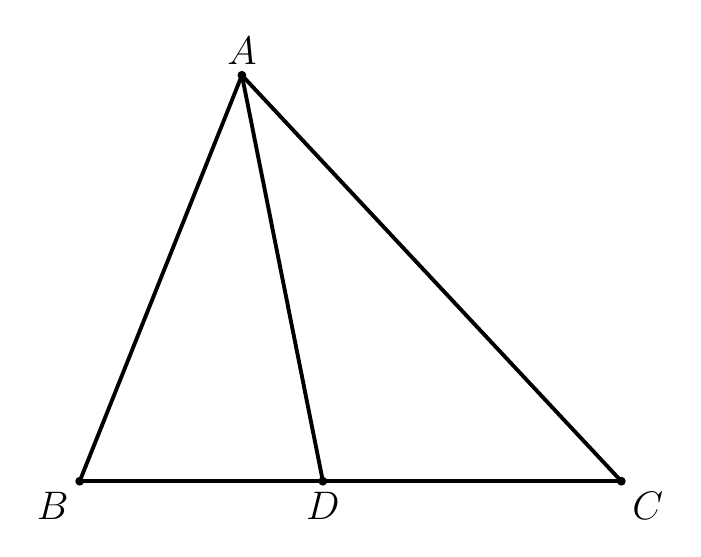
\begin{tikzpicture}[line join=round, line width=1.4pt]
\coordinate (A) at (-1.384,2.582);
\coordinate (B) at (-3.444,-2.573);
\coordinate (C) at (3.434,-2.573);
\coordinate (D) at (-0.356,-2.573);

  
  \draw (A) -- (B);
  \draw (A) -- (C);
  
  \draw (B) -- (D) -- (C);
  
  \draw (A) -- (D);

  
  \fill (A) circle (1.600pt);
  \fill (B) circle (1.600pt);
  \fill (C) circle (1.600pt);
  \fill (D) circle (1.600pt);

  
  \node[above] at (A) {\fontsize{15}{18}\selectfont $A$};
  \node[below left] at (B) {\fontsize{15}{18}\selectfont $B$};
  \node[below right] at (C) {\fontsize{15}{18}\selectfont $C$};
  \node[below] at (D) {\fontsize{15}{18}\selectfont $D$};
\end{tikzpicture}
\end{document}